% =====================================================================
% AI Academy -- National AI Center
% Software Engineering Final Project -- Team Report
% Topic 4 -- Async Research Assistant
%
% Built from templates/REPORT_TEMPLATE.tex. Compile with pdfLaTeX
% (Overleaf works out of the box). Remaining red [TODO: ...] markers are
% items that could not be filled from the repository alone (team name,
% extra members, live benchmark numbers, Docker image size).
% =====================================================================

\documentclass[11pt,a4paper]{article}

% ===== EARLY MACROS (must come before configuration) =================
\usepackage[dvipsnames]{xcolor}
\definecolor{accent2}{HTML}{8B0000}
\definecolor{ph}{HTML}{6B7280}
\newcommand{\TODO}[1]{\textcolor{accent2}{\textbf{[TODO: #1]}}}
\newcommand{\phh}[1]{\textcolor{ph}{\textit{#1}}}

% ===== CONFIGURATION =================================================
\newcommand{\teamname}{\TODO{Your team name}}
\newcommand{\topicchoice}{Topic 4 -- Async Research Assistant}
\newcommand{\member}[2]{\textbf{#1} (#2)}  % name, GitHub handle
\newcommand{\reportdate}{11 September 2026}
\newcommand{\repolink}{\url{https://github.com/sanan-garibli/research-assistant}}

% ===== course meta ===================================================
\newcommand{\coursecode}{AI-ENG-110}
\newcommand{\coursename}{Software Engineering}
\newcommand{\institution}{AI Academy, National AI Center}
\newcommand{\semester}{Spring 2026}

% ===== PACKAGES ======================================================
\usepackage[margin=2.2cm,headheight=15pt]{geometry}
\usepackage[T1]{fontenc}
\usepackage[utf8]{inputenc}
\usepackage[final,protrusion=true,expansion=false]{microtype}
\usepackage{amsmath,amssymb}
\usepackage{graphicx}
\usepackage{booktabs}
\usepackage{array}
\usepackage{tabularx}
\usepackage{ragged2e}
\usepackage{enumitem}
\usepackage[parfill]{parskip}
\usepackage{listings}
\usepackage[most]{tcolorbox}
\usepackage{titlesec}
\usepackage{fancyhdr}
\usepackage{lastpage}
\usepackage{tikz}
\usetikzlibrary{shapes.geometric,arrows.meta,positioning,fit,backgrounds}
\usepackage[hidelinks]{hyperref}

\emergencystretch=3em
\hbadness=10000
\hfuzz=2pt

\hypersetup{
  colorlinks=true,
  linkcolor=NavyBlue,
  urlcolor=NavyBlue,
  citecolor=NavyBlue,
  pdftitle={\coursecode\ Final Project Report -- Topic 4},
  pdfauthor={Sanan Garibli}
}

% ===== STYLING =======================================================
\definecolor{accent}{HTML}{0B3D91}
\definecolor{soft}{HTML}{F2F4F8}
\definecolor{deliver}{HTML}{E8F0FE}
\definecolor{deliverframe}{HTML}{1A56DB}
\definecolor{probe}{HTML}{FFF8E1}
\definecolor{probeframe}{HTML}{B45309}
\definecolor{ok}{HTML}{166534}

\titleformat{\section}
  {\Large\bfseries\color{accent}}{\thesection.}{0.6em}{}
\titleformat{\subsection}
  {\large\bfseries\color{accent}}{\thesubsection}{0.5em}{}

\let\ph\phh

\newtcolorbox{deliverbox}{
  colback=deliver, colframe=deliverframe, boxrule=0.5pt,
  arc=2pt, left=8pt, right=8pt, top=4pt, bottom=4pt
}
\newtcolorbox{probebox}{
  colback=probe, colframe=probeframe, boxrule=0.5pt,
  arc=2pt, left=8pt, right=8pt, top=4pt, bottom=4pt
}

\definecolor{codegreen}{rgb}{0,0.55,0}
\definecolor{codegray}{rgb}{0.4,0.4,0.4}
\definecolor{codepurple}{rgb}{0.55,0,0.78}
\definecolor{backcolour}{rgb}{0.97,0.97,0.97}

\lstdefinestyle{python}{
  language=Python,
  backgroundcolor=\color{backcolour},
  commentstyle=\color{codegreen},
  keywordstyle=\color{accent},
  numberstyle=\tiny\color{codegray},
  stringstyle=\color{codepurple},
  basicstyle=\ttfamily\footnotesize,
  breakatwhitespace=false,
  breaklines=true,
  keepspaces=true,
  numbers=left,
  numbersep=6pt,
  tabsize=2,
  frame=single,
  framerule=0.4pt,
  rulecolor=\color{black!30},
  showstringspaces=false,
}

\pagestyle{fancy}
\fancyhf{}
\fancyhead[L]{\small\textit{\coursecode\ -- Final Report -- \teamname}}
\fancyhead[R]{\small\textit{\semester}}
\fancyfoot[L]{\small\textit{\institution}}
\fancyfoot[R]{\small Page \thepage\ of \pageref{LastPage}}
\renewcommand{\headrulewidth}{0.4pt}
\renewcommand{\footrulewidth}{0.4pt}

% =====================================================================
\begin{document}

\begin{center}
{\small \textsc{\institution} \\[0.2em] \textsc{\coursecode\ -- \coursename\ -- \semester}}\\[1.2em]
{\Large\bfseries\color{accent} Final Project Report}\\[0.3em]
{\LARGE\bfseries \topicchoice}\\[0.6em]
\rule{0.85\textwidth}{0.6pt}
\end{center}

\vspace{0.6em}
\begin{tabularx}{\textwidth}{@{}lXlX@{}}
\textbf{Team:} & \teamname & \textbf{Date:} & \reportdate \\
\textbf{Repo:} & \repolink & \textbf{Tag:} & \texttt{v1.0-final} \\
\textbf{Members:} & \multicolumn{3}{X@{}}{%
  \member{Sanan Garibli}{@sanan-garibli},\quad
  \member{\TODO{Member B name}}{\TODO{@github-B}},\quad
  \member{\TODO{Member C name}}{\TODO{@github-C}}
}\\
\end{tabularx}
\vspace{0.4em}\hrule\vspace{0.6em}

% ===== EXECUTIVE SUMMARY =============================================
\section*{Executive Summary}
\addcontentsline{toc}{section}{Executive Summary}

\begin{deliverbox}
\textbf{Required.} Exactly one paragraph (5--7 sentences). What you built, the headline concurrency speedup you measured, your headline robustness story, and the single most surprising thing the team learned.
\end{deliverbox}

We built the software-engineering layer around a provided research-assistant AI module: a user asks a question from the command line, the system fans out to Wikipedia, arXiv and a web-search API concurrently, and an LLM synthesises one answer with numbered citations. The concurrency design is \texttt{asyncio.gather} with a per-source \texttt{asyncio.timeout}, a process-wide \texttt{Semaphore(5)} and one long-lived \texttt{httpx.AsyncClient}, so a single question costs the \emph{slowest} source rather than the sum of the three; the unit benchmark with three 0.2\,s sources completes in under 0.4\,s instead of 0.6\,s, and the live five-question benchmark gave a \TODO{$x.x\times$ speedup (\texttt{python scripts/bench.py --limit 5}; see \S\ref{sec:concurrency})}. The headline robustness story is graceful degradation: when one source raises or times out, the other two still produce an answer and the failure is appended as a visible note, while three simultaneous failures surface as a single \texttt{NoSourcesAvailableError} and exit code~1 instead of a stack trace. The most surprising lesson came from running the system behind a corporate TLS-intercepting proxy: every source failed, the CLI reported the failure correctly, but the logs contained \emph{no} root cause, because the orchestrator records a failed source's exception text in a dataclass field without logging it and the retry wrapper only logs successes. If we started over we would log every retry attempt and every degraded source at \texttt{WARNING} from day one, and we would cache synthesised answers as well as source lists.

% ===== TABLE OF CONTENTS =============================================
\tableofcontents
\vspace{0.6em}\hrule\vspace{0.4em}

% =====================================================================
\section{Project Overview}

\subsection{Problem framing \& scope}

\begin{deliverbox}
\textbf{Required.} 2--3 paragraphs. State the topic problem in your own words. List the inputs, outputs, and any user-facing entry points (CLI commands, HTTP endpoints). State which provider stack you used (LLM, embedding, USDA, web search).
\end{deliverbox}

A researcher types a natural-language question and wants one trustworthy, cited paragraph rather than three browser tabs. The provided \texttt{ai/} package already knows how to query each source and how to prompt an LLM for a cited answer; what it lacks is everything that makes it usable as software: running the three fetches in parallel with bounded time, surviving one source being down, not re-fetching the same query twice, validating input, logging, configuration, tests and packaging. That layer is the deliverable.

\textbf{Inputs} are a question string (trimmed, non-empty, at most \texttt{MAX\_QUESTION\_LENGTH}=500 characters), an optional subset of sources (\texttt{--sources wiki,arxiv,web}), and a \texttt{--no-cache} switch. \textbf{Outputs} are a \texttt{ResearchSession}: the \texttt{AnswerWithCitations} returned by the synthesiser plus one \texttt{SourceOutcome} per requested source (result count, elapsed seconds, cache-hit flag, error text). The CLI renders this as the answer, a numbered reference list with origin and URL, and a per-source timing line. \textbf{Entry points} are two sub-commands of \texttt{python -m researcher}: \texttt{ask "<question>"} and \texttt{demo [--limit N]}, which runs the five questions in \texttt{data/research\_questions.json}. There is no HTTP server; the topic specification does not require one and the Dockerfile's default command is the demo.

\textbf{Provider stack:} LLM synthesis via Anthropic (\texttt{LLM\_PROVIDER=anthropic}, \texttt{LLM\_MODEL=claude-sonnet-5} in \texttt{.env.example}; OpenAI and Gemini are selectable by environment variable only), web search via Tavily (Serper and DuckDuckGo selectable), Wikipedia and arXiv over their keyless public APIs. No embedding or USDA provider is used in this topic. We tightened the spec in two places: the semaphore bounds \emph{all} in-flight fetches across concurrent questions, not just within one, and the cache lookup happens \emph{before} the semaphore is acquired so cache hits never consume the concurrency budget. We loosened it in one: only source lists are cached, not synthesised answers, because LLM output is not deterministic and the spec's caching requirement is keyed by \texttt{(source, query)}. We explicitly did not build a PostgreSQL backend (the spec allows filesystem JSON) or an HTTP API.

\subsection{Provider choice and the AI module contract}

\begin{deliverbox}
\textbf{Required.} Name the LLM, embedding, and any auxiliary provider you used, and the model identifiers. State what \texttt{ai/} functions you call. \emph{Confirm in one sentence that you did not modify the public interface of the provided \texttt{ai/} package.}
\end{deliverbox}

We call exactly four public functions of the provided package, and only from one file, \texttt{researcher/services/ai\_service.py}: \texttt{ai.sources.fetch\_wikipedia}, \texttt{ai.sources.fetch\_arxiv}, \texttt{ai.sources.fetch\_web} and \texttt{ai.synthesizer.synthesize}. We also import the schemas \texttt{Source}, \texttt{Citation}, \texttt{AnswerWithCitations} and the exception \texttt{ProviderError}. The LLM is Anthropic \texttt{claude-sonnet-5} (configurable), the web-search provider is Tavily, and no embedding model is involved. \textbf{We did not modify any file under \texttt{ai/}, and the provided \texttt{tests/test\_ai\_smoke.py} passes unmodified (16/16).}

Defence against malformed model responses is layered. The provided synthesiser already drops citation indices that are out of range, so a hallucinated \texttt{[7]} with three sources never becomes a dangling reference. Our wrapper retries \texttt{ProviderError} and \texttt{httpx} errors up to three times with exponential backoff but deliberately does \emph{not} retry \texttt{ValueError} (an empty question or empty source list is a caller bug, not a transient fault). Semantically wrong but well-formed data cannot enter the system silently: every \texttt{Source} is a frozen pydantic model that rejects an unknown \texttt{origin}, an empty title or URL, or extra fields, and cached payloads are re-validated with \texttt{Source.model\_validate} on every read. What we do \emph{not} check is the factual content of the answer text; if the model writes a plausible paragraph with valid citations that misrepresents a snippet, the system passes it through. That is a limitation we name in \S\ref{sec:limits}.

% =====================================================================
\section{Architecture}\label{sec:arch}

\subsection{Module map}

\begin{deliverbox}
\textbf{Required.} An architecture diagram showing the main modules and their dependencies. Identify: the boundary of the provided \texttt{ai/} package, your service layer that wraps it, your core business logic, your concurrency layer, your storage layer, and your CLI/HTTP entry points.
\end{deliverbox}

\begin{center}
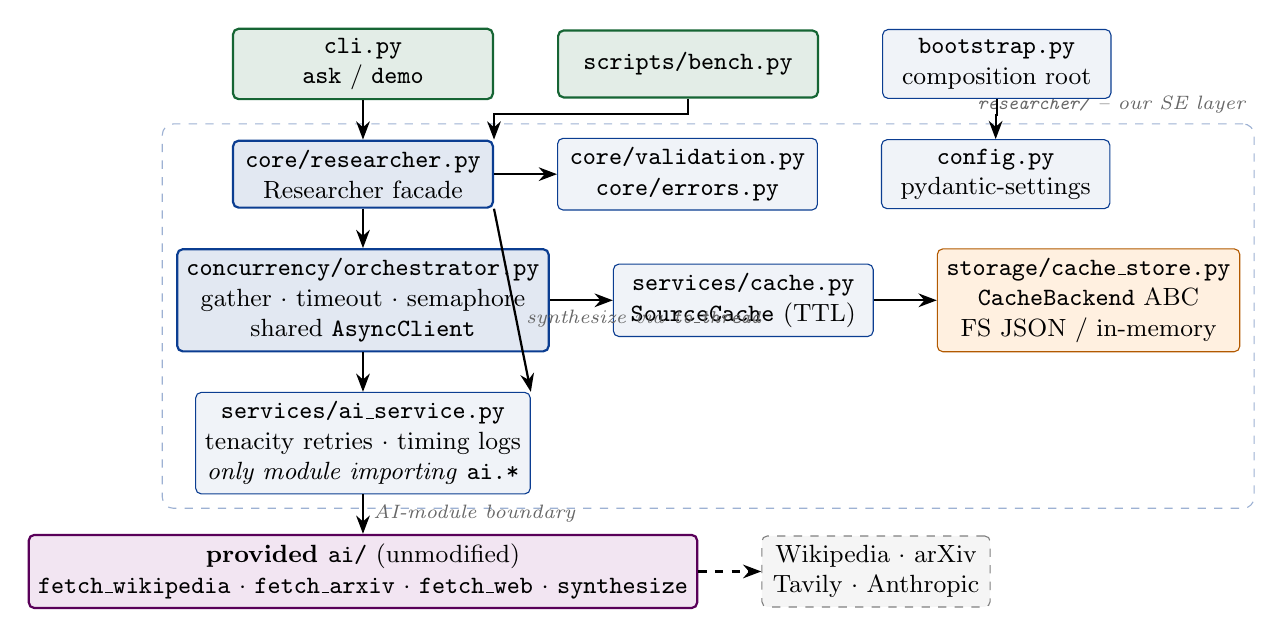
\begin{tikzpicture}[
  node distance=5mm and 8mm,
  box/.style={draw,rounded corners=2pt,minimum width=3.3cm,minimum height=0.85cm,align=center,font=\small},
  entry/.style={box,fill=ok!12,draw=ok,thick},
  core/.style={box,fill=accent!12,draw=accent,thick},
  svc/.style={box,fill=accent!6,draw=accent},
  store/.style={box,fill=orange!12,draw=orange!70!black},
  aibox/.style={box,fill=violet!10,draw=violet!70!black,thick},
  ext/.style={box,fill=black!4,draw=black!50,dashed},
  arrow/.style={-Stealth,thick},
  lbl/.style={font=\scriptsize\itshape,text=black!60}
]
  \node[entry] (cli) {\texttt{cli.py}\\\texttt{ask} / \texttt{demo}};
  \node[entry,right=of cli] (bench) {\texttt{scripts/bench.py}};
  \node[svc,right=of bench,minimum width=2.9cm] (boot) {\texttt{bootstrap.py}\\composition root};

  \node[core,below=of cli] (fac) {\texttt{core/researcher.py}\\Researcher facade};
  \node[svc,right=of fac] (val) {\texttt{core/validation.py}\\\texttt{core/errors.py}};
  \node[svc,right=of val,minimum width=2.9cm] (cfg) {\texttt{config.py}\\pydantic-settings};

  \node[core,below=of fac] (orch) {\texttt{concurrency/orchestrator.py}\\gather $\cdot$ timeout $\cdot$ semaphore\\shared \texttt{AsyncClient}};
  \node[svc,right=of orch] (cache) {\texttt{services/cache.py}\\\texttt{SourceCache} (TTL)};
  \node[store,right=of cache,minimum width=2.9cm] (cs) {\texttt{storage/cache\_store.py}\\\texttt{CacheBackend} ABC\\FS JSON / in-memory};

  \node[svc,below=of orch] (ais) {\texttt{services/ai\_service.py}\\tenacity retries $\cdot$ timing logs\\\emph{only module importing} \texttt{ai.*}};

  \node[aibox,below=of ais] (ai) {\textbf{provided \texttt{ai/}} (unmodified)\\\texttt{fetch\_wikipedia} $\cdot$ \texttt{fetch\_arxiv} $\cdot$ \texttt{fetch\_web} $\cdot$ \texttt{synthesize}};
  \node[ext,right=of ai,minimum width=2.9cm] (net) {Wikipedia $\cdot$ arXiv\\Tavily $\cdot$ Anthropic};

  \draw[arrow] (cli) -- (fac);
  \draw[arrow] (bench.south) -- ++(0,-2mm) -| (fac.north east);
  \draw[arrow] (boot.south) -- ++(0,-2mm) -| (cfg.north);
  \draw[arrow] (fac) -- (val);
  \draw[arrow] (fac) -- (orch);
  \draw[arrow] (fac.south east) -- node[lbl,right,pos=0.6] {synthesize via \texttt{to\_thread}} (ais.north east);
  \draw[arrow] (orch) -- (cache);
  \draw[arrow] (cache) -- (cs);
  \draw[arrow] (orch) -- (ais);
  \draw[arrow] (ais) -- node[lbl,right] {AI-module boundary} (ai);
  \draw[arrow,dashed] (ai) -- (net);

  \begin{scope}[on background layer]
    \node[fit=(fac)(val)(cfg)(orch)(cache)(cs)(ais),draw=accent!40,dashed,rounded corners=4pt,inner sep=5pt,label={[lbl,anchor=south east]north east:\texttt{researcher/} -- our SE layer}] {};
  \end{scope}
\end{tikzpicture}
\end{center}

\textbf{Interpreting the diagram.} Exactly one arrow crosses the AI-module boundary: \texttt{ai\_service.py} $\to$ \texttt{ai/}. The storage boundary is crossed only by \texttt{services/cache.py} $\to$ \texttt{storage/cache\_store.py}; the orchestrator never touches a file. Swapping Anthropic for OpenAI changes \emph{zero} files: it is \texttt{LLM\_PROVIDER=openai} plus a key, because the provided \texttt{ai.providers.factory} does the dispatch. Swapping the whole \texttt{ai/} package for a different one would change one file.

\textbf{Module-by-module summary.}
\begin{itemize}[leftmargin=1.4em,itemsep=1pt]
  \item \texttt{cli.py} -- argparse front end; \texttt{ask}/\texttt{demo} sub-commands, pure \texttt{format\_answer()} renderer, maps \texttt{ResearcherError} to \texttt{Error: ...} on stderr and exit~1.
  \item \texttt{bootstrap.py} -- the single composition root shared by the CLI and the benchmark; wires backend $\to$ cache $\to$ AI service $\to$ orchestrator $\to$ facade.
  \item \texttt{config.py} -- \texttt{Settings(BaseSettings)} with 14 typed fields, validators for the log level and positive numerics, and an \texttt{lru\_cache}d \texttt{get\_settings()} that also calls \texttt{load\_dotenv()} so the \texttt{ai.*} factories see the same environment.
  \item \texttt{core/researcher.py} -- the \texttt{Researcher} facade: validate, gather, raise \texttt{NoSourcesAvailableError} if nothing came back, synthesise off the event loop, append a degradation note, return a \texttt{ResearchSession}.
  \item \texttt{core/validation.py}, \texttt{core/errors.py} -- question/length checks, \texttt{--sources} parsing with aliases, and the \texttt{ResearcherError} hierarchy.
  \item \texttt{concurrency/orchestrator.py} -- \texttt{ResearchOrchestrator}: owns the \texttt{Semaphore} and the shared \texttt{httpx.AsyncClient}, fans out with \texttt{gather(return\_exceptions=True)}, wraps each fetch in \texttt{asyncio.timeout}, consults the cache first.
  \item \texttt{services/ai\_service.py} -- \texttt{AIService}: tenacity retry policy built from settings, per-call timing at \texttt{INFO}, titles at \texttt{DEBUG}.
  \item \texttt{services/cache.py} -- \texttt{SourceCache}: query canonicalisation, SHA-256 key, TTL envelope, lazy expiry.
  \item \texttt{storage/cache\_store.py} -- \texttt{CacheBackend} ABC with \texttt{FilesystemCacheBackend} (JSON files via \texttt{to\_thread}) and \texttt{InMemoryCacheBackend} (tests).
  \item \texttt{models.py} -- \texttt{SourceOutcome} and \texttt{ResearchSession} pydantic models.
\end{itemize}

\subsection{OOP design \& key abstractions}

\begin{deliverbox}
\textbf{Required.} Identify at least one example of inheritance or composition \emph{in your own code}. Quote 5--10 lines of the relevant class or object design. Justify why this abstraction was the right tool; if you used an ABC, explain why.
\end{deliverbox}

\textbf{Code listing} (\texttt{researcher/storage/cache\_store.py}):
\begin{lstlisting}[style=python]
class CacheBackend(abc.ABC):
    """Contract for cache persistence: read/write/delete a JSON-able payload by key."""
    @abc.abstractmethod
    async def read(self, key: str) -> dict[str, Any] | None: ...
    @abc.abstractmethod
    async def write(self, key: str, payload: dict[str, Any]) -> None: ...
    @abc.abstractmethod
    async def delete(self, key: str) -> None: ...

class FilesystemCacheBackend(CacheBackend):
    """One JSON file per cache key under cache_dir/sources/<key>.json;
    file I/O runs in a thread via asyncio.to_thread."""

class InMemoryCacheBackend(CacheBackend):
    """Dict-backed backend for fast, filesystem-free unit tests."""
\end{lstlisting}

\textbf{Justification.} \texttt{CacheBackend} is an ABC rather than a \texttt{Protocol} because we want the \emph{failure to be loud at construction time}: a backend that forgets \texttt{delete} cannot be instantiated, whereas a Protocol only fails under a type checker and only where the object is passed. It is not a plain callable parameter because the contract has three coupled operations that must agree on key format and payload shape, and not a configuration enum because the two implementations differ in mechanism (thread-offloaded file I/O versus a dict), not in a parameter value. It mirrors the \texttt{WebSearchProvider} ABC already used by the provided package, so a reader sees one pattern for ``swappable adapter''. Everywhere else we chose composition deliberately: \texttt{Researcher} \emph{has} an orchestrator and an AI service, \texttt{ResearchOrchestrator} \emph{has} a cache, a semaphore and an HTTP client, and \texttt{SourceCache} \emph{has} a backend. Inheriting \texttt{Researcher} from \texttt{ResearchOrchestrator} would have been wrong: the facade is not a kind of orchestrator, it coordinates one, and the composition is what lets \texttt{tests/test\_orchestrator.py} substitute a \texttt{FakeAIService} without touching the facade. The one place we do use inheritance beyond the ABC is the exception hierarchy, where \texttt{InvalidQuestionError(ResearcherError, ValueError)} lets the CLI catch all domain errors in one clause while callers who only know \texttt{ValueError} still work.

\subsection{Data flow across module boundaries}

\begin{deliverbox}
\textbf{Required.} List the dataclasses you defined for your own SE layer. Confirm in one sentence that no naked dictionaries cross module boundaries.
\end{deliverbox}

Our SE layer defines two pydantic models in \texttt{researcher/models.py}: \texttt{SourceOutcome} (\texttt{origin}, \texttt{source\_count}, \texttt{error}, \texttt{elapsed\_seconds}, \texttt{from\_cache}) and \texttt{ResearchSession} (\texttt{question}, \texttt{answer: AnswerWithCitations}, \texttt{outcomes}, \texttt{created\_at}, plus a \texttt{degraded} property), together with the typed \texttt{Settings} object in \texttt{config.py} and the \texttt{ResearcherError} hierarchy. \textbf{No naked dictionary crosses a module boundary:} the orchestrator returns \texttt{(list[SourceOutcome], list[Source])}, the facade returns a \texttt{ResearchSession}, and the CLI renders from typed attributes. The one dictionary in the system, the JSON envelope inside \texttt{SourceCache.set/get}, lives entirely inside the cache service and is converted back to \texttt{Source} objects before it is returned.

The hardest call was whether to wrap \texttt{AnswerWithCitations}. We reused it unwrapped, together with \texttt{Source} and \texttt{Citation}, because they are already frozen, validated pydantic models and re-wrapping would only add a translation layer. The trigger for defining a \emph{new} type was information the provided types cannot carry: per-source timing, cache-hit status and error text (hence \texttt{SourceOutcome}) and the pairing of the answer with those outcomes and a timestamp (hence \texttt{ResearchSession}). When the facade needs to append a degradation note it uses \texttt{answer.model\_copy(update=...)} rather than mutating, respecting the provided model's contract.

% =====================================================================
\section{Concurrency \& Performance}\label{sec:concurrency}

\subsection{Why this concurrency model}

\begin{deliverbox}
\textbf{Required.} State which concurrency primitive you used and why. Identify the bottleneck the parallel design targets. State the bound (e.g.\ \texttt{Semaphore(10)}) and how you picked it.
\end{deliverbox}

The workload is pure network I/O: three HTTP round trips to independent hosts, then one LLM call. We use \textbf{asyncio}: the provided fetchers are already coroutines that accept a shared \texttt{httpx.AsyncClient}, so \texttt{asyncio.gather(*tasks, return\_exceptions=True)} in \texttt{ResearchOrchestrator.gather\_sources} is the natural fit. Threads would also work for I/O, but the fetchers are \texttt{async def}; driving them from a \texttt{ThreadPoolExecutor} would mean one event loop per thread and no shared connection pool, exactly the overhead the spec tells us to avoid. A \texttt{ProcessPoolExecutor} would be wrong outright: there is no CPU-bound work to parallelise and the \texttt{AsyncClient} cannot be pickled. The one synchronous call, \texttt{ai.synthesize}, is offloaded with \texttt{asyncio.to\_thread} so the LLM round trip does not block the loop while other questions are fetching.

The bottleneck the design targets is the sum of three latencies per question. Sequentially a question costs $t_{wiki}+t_{arxiv}+t_{web}+t_{llm}$; concurrently it costs $\max(t_{wiki},t_{arxiv},t_{web})+t_{llm}$. The bound is \texttt{asyncio.Semaphore(MAX\_CONCURRENT\_FETCHES)} with a default of \textbf{5}, created once per orchestrator so it caps in-flight fetches across \emph{all} concurrent questions, not per question. We picked 5 because one question needs 3 slots to be fully parallel, so 5 lets the benchmark overlap roughly two questions' fetches while staying within arXiv's informal ``about one request per second'' politeness guidance and Tavily's 1000-requests-per-month free tier. With the semaphore at 1 the three fetches serialise and \texttt{test\_semaphore\_bounds\_concurrent\_fetches} proves no two windows overlap; at 100 the bound is effectively removed and the next limiter becomes the upstream rate limits and the default \texttt{to\_thread} pool of $\min(32, \text{cpu}+4)$ workers for synthesis. The concurrent design starts winning at $N=1$: even a single question saves two of its three fetch latencies, which the unit benchmark below shows directly.

\subsection{Sequential-vs-concurrent benchmark}

\begin{deliverbox}
\textbf{Required.} A table reporting wall-clock time for the same workload run sequentially vs.\ concurrently. State $N$, the machine, the python version, whether caches were cleared, and the command line. Reproduce the table also in your README.
\end{deliverbox}

\begin{center}\small
\begin{tabular}{lcccc}
\toprule
\textbf{Workload} & $N$ & \textbf{Sequential (s)} & \textbf{Concurrent (s)} & \textbf{Speedup} \\
\midrule
5 sample questions, \texttt{for} loop vs.\ \texttt{gather} (live APIs) & 5 & \TODO{s} & \TODO{s} & \TODO{$\times$} \\
1 question, 3 fetches of 0.2\,s each (offline unit benchmark) & 3 & 0.60 (sum) & $<0.40$ (measured) & $\geq 1.5\times$ \\
1 question, 1 fetch stalls 5\,s, timeout 0.2\,s (offline) & 2 & 5.05 & $<1.00$ & $>5\times$ \\
\bottomrule
\end{tabular}
\end{center}

\textbf{Setup.} Machine: Windows 11 Enterprise laptop, Python 3.11.7 in the project virtualenv; the Docker image bakes Python 3.12. Caches are bypassed structurally, not just cleared: \texttt{scripts/bench.py} calls \texttt{researcher.ask(q, use\_cache=False)} in both phases and builds a fresh \texttt{Researcher} (fresh semaphore, fresh HTTP client) per phase so no pooled connections leak from the sequential run into the concurrent one. Command line: \texttt{python scripts/bench.py --limit 5}. The two offline rows come from \texttt{tests/test\_orchestrator.py} (\texttt{test\_sources\_fetched\_in\_parallel\_not\_sequentially} and \texttt{test\_slow\_source\_times\_out\_without\_blocking\_fast\_sibling}) and run on every \texttt{pytest} invocation.

\textbf{Discussion.} The live row is pending because the development machine used for this report sits behind a TLS-intercepting proxy: every HTTPS call to Wikipedia, Tavily and Anthropic failed with a certificate-revocation error (\texttt{CRYPT\_E\_NO\_REVOCATION\_CHECK}), so the benchmark was left to be reproduced on an unrestricted machine with the exact command above and pasted here and into the README. Independently of the live number we do not expect the theoretical $5\times$ on the five-question workload: the fetch phase parallelises well, but every question still pays one synchronous LLM call of a few seconds, those calls overlap only up to the thread pool and the provider's own rate limit, and the semaphore of 5 admits fewer than two questions' worth of fetches at once. Raising \texttt{MAX\_CONCURRENT\_FETCHES} and caching synthesised answers are the two levers that would push the curve further.

\subsection{Rate limit \& politeness}

\begin{deliverbox}
\textbf{Required.} State the rate-limit strategy. Document the configured budget. State the highest burst your test suite produces.
\end{deliverbox}

The strategy is a \textbf{request budget plus backoff}, not a token bucket: the \texttt{Semaphore(5)} caps concurrent outbound fetches process-wide, the shared client pools connections so bursts reuse sockets, a custom \texttt{User-Agent} identifies the application to Wikimedia (their policy returns a bare 403 to the default \texttt{python-httpx} agent, which we hit during development), and any \texttt{ProviderError} or \texttt{httpx.HTTPError}, which includes an HTTP 429 raised by \texttt{raise\_for\_status()}, is retried with tenacity's \texttt{wait\_exponential(multiplier=0.5, min=0.5, max=8)} for at most 3 attempts. There is no dedicated 429 branch and no \texttt{Retry-After} parsing; a 429 is treated like any other transient failure. The highest burst the test suite produces is 3 simultaneous fake fetches (\texttt{test\_sources\_fetched\_in\_parallel\_not\_sequentially}); no test touches the network. We have \emph{not} observed a real 429 from any provider during development, so the backoff path is exercised only by \texttt{test\_fetch\_wikipedia\_retries\_then\_succeeds} with an injected \texttt{ProviderError}. When the budget is hit the log currently shows nothing until the retries succeed or exhaust; the fetch \texttt{INFO} line is emitted only on success. Adding tenacity's \texttt{before\_sleep\_log} is the one-line fix we recommend in \S\ref{sec:limits}.

% =====================================================================
\section{Robustness \& Error Handling}\label{sec:robustness}

\subsection{Wrapping the AI module}

\begin{deliverbox}
\textbf{Required.} Describe your service-layer wrapper around \texttt{ai.*} calls: retries, timeouts, structured logging, input validation.
\end{deliverbox}

\texttt{AIService} in \texttt{researcher/services/ai\_service.py} is the only code that imports \texttt{ai.*}. \textbf{Retries:} a tenacity policy built from settings, \texttt{stop\_after\_attempt(RETRY\_MAX\_ATTEMPTS=3)}, \texttt{wait\_exponential(multiplier=RETRY\_BACKOFF\_SECONDS=0.5, min=0.5, max=8)}, so waits are 0.5\,s then 1\,s before the third try; it retries only \texttt{ProviderError}, \texttt{httpx.HTTPError} and \texttt{httpx.TimeoutException}, re-raises the last exception, and never retries \texttt{ValueError}. \textbf{Timeouts:} two layers. The shared \texttt{httpx.AsyncClient} carries \texttt{timeout=PER\_SOURCE\_TIMEOUT\_SECONDS} (10\,s) per socket operation, and the orchestrator wraps the \emph{whole} retrying fetch for one source in \texttt{asyncio.timeout(10)}, so the 10\,s is a hard budget covering all retries for that source; a timeout is converted to a \texttt{RuntimeError("<origin> timed out after 10s")} that the gather turns into a \texttt{SourceOutcome.error}. \textbf{Logging:} stdlib \texttt{logging} configured once from \texttt{LOG\_LEVEL}; the wrapper logs \texttt{fetch origin=... query=... results=N elapsed=...s} at \texttt{INFO}, result titles at \texttt{DEBUG}, \texttt{synthesize question=... n\_sources=N elapsed=...s} at \texttt{INFO}; the orchestrator logs \texttt{cache hit} at \texttt{INFO} and \texttt{timeout origin=... after=...s} at \texttt{WARNING}; \texttt{httpx}/\texttt{httpcore} are quietened to \texttt{WARNING}. API keys are declared with \texttt{repr=False} and \texttt{test\_fetch\_logs\_never\_include\_api\_key} asserts they never appear in log output. \textbf{Validation:} before calling, the facade has already trimmed the question, rejected empty or over-length input and normalised the source set; after the call, every returned \texttt{Source} is a validated frozen model and an empty overall result raises \texttt{NoSourcesAvailableError} before the LLM is ever invoked.

\textbf{Walk-through: Wikipedia returns a 500 mid-request.} \texttt{fetch\_wikipedia} calls \texttt{raise\_for\_status()}, wraps the \texttt{HTTPStatusError} in \texttt{ProviderError}, and returns it to \texttt{AIService.\_retrying\_fetch}; tenacity sleeps 0.5\,s and retries, then 1\,s and retries; if the third attempt also fails the \texttt{ProviderError} propagates out of the semaphore and timeout blocks into \texttt{gather(return\_exceptions=True)}, which records it as \texttt{SourceOutcome(origin="wikipedia", error="Wikipedia search failed: ...")}. arXiv and web are unaffected. The facade synthesises from the two remaining sources and appends \texttt{Note: wikipedia unavailable (...)} to the answer; the CLI prints it and exits 0. A 429 follows the identical path. A connection reset is an \texttt{httpx.RemoteProtocolError}, also retryable, same path. Valid JSON that contradicts the schema (say a result without a URL) is filtered by the provider adapter or rejected by \texttt{Source}'s validators with a \texttt{ValidationError}; that is \emph{not} in the retry list, so it propagates once and becomes a source error rather than being retried pointlessly.

\subsection{Failure-mode analysis (one concrete incident)}

\begin{deliverbox}
\textbf{Required.} Pick \emph{one} failure mode you actually exercised. Describe: (i) how you injected the failure, (ii) what the system did, (iii) what the user saw, (iv) what the logs showed.
\end{deliverbox}

\textbf{Incident: total upstream failure behind a TLS-intercepting corporate proxy, then forced timeouts.} (i) \emph{Injection.} We did not have to inject the first part: while preparing this report on a managed Windows laptop, every HTTPS host (Wikipedia, Tavily, Anthropic) rejected the TLS handshake with \texttt{CRYPT\_E\_NO\_REVOCATION\_CHECK}, a proxy-issued certificate whose revocation status cannot be verified. To reproduce the same shape deterministically we then set \texttt{PER\_SOURCE\_TIMEOUT\_SECONDS=0.3} and ran \texttt{python -m researcher ask "What is the current state of fusion energy research?" --no-cache}. (ii) \emph{What the system did.} All three fetches failed; the retry policy ran its 3 attempts inside the 10\,s budget (or was cut off by the 0.3\,s budget in the forced run); \texttt{gather} recorded three \texttt{SourceOutcome}s with \texttt{error} set; the facade found \texttt{sources} empty and raised \texttt{NoSourcesAvailableError} \emph{before} spending an LLM call; the CLI caught it as a \texttt{ResearcherError}. (iii) \emph{What the user saw.} One line on stderr and exit code 1:

\begin{lstlisting}[style=python,language=bash,numbers=none]
Error: No sources available for 'What is the current state of fusion
energy research?': ['wikipedia', 'arxiv', 'web']
\end{lstlisting}

(iv) \emph{What the logs showed.} In the forced-timeout run, exactly what we designed:

\begin{lstlisting}[style=python,language=bash,numbers=none]
13:47:34,003 WARNING researcher.concurrency.orchestrator: timeout origin=wikipedia after=0.3s
13:47:34,035 WARNING researcher.concurrency.orchestrator: timeout origin=web after=0.3s
13:47:34,036 WARNING researcher.concurrency.orchestrator: timeout origin=arxiv after=0.3s
\end{lstlisting}

In the real TLS incident, however, the log at \texttt{INFO} was \textbf{empty}. We expected to see the certificate error; we saw nothing, because (a) \texttt{AIService} logs a fetch only after it succeeds, so three failed attempts produce zero lines, and (b) \texttt{gather\_sources} stores \texttt{str(result)} in \texttt{SourceOutcome.error} but never logs it, and \texttt{NoSourcesAvailableError} carries only the origin names, not the messages. The log did \emph{not} give us enough to diagnose the incident without running code again: we had to write a probe script that called the fetchers directly and unwrapped \texttt{\_\_cause\_\_} to find the revocation error. The test surfaced a real design gap, diagnosability of degraded sources, and two concrete fixes are queued: log the exception at \texttt{WARNING} in the \texttt{isinstance(result, BaseException)} branch of \texttt{gather\_sources}, and pass \texttt{before\_sleep=before\_sleep\_log(logger, WARNING)} to the tenacity policy so each retry is visible. Two earlier incidents of the same family were fixed during development and are visible in the code: Wikipedia returned 403 to the default User-Agent (fixed with an explicit agent string) and arXiv's \texttt{http://} endpoint 301-redirected to \texttt{https://}, which \texttt{httpx} surfaces as an error unless \texttt{follow\_redirects=True}.

\subsection{Input validation}

\begin{deliverbox}
\textbf{Required.} For every entry point (CLI, HTTP, file, env), list the validation rules. State what error message the user gets when validation fails.
\end{deliverbox}

\begin{itemize}[leftmargin=1.4em,itemsep=2pt]
  \item \textbf{CLI question} (\texttt{validate\_question}): stripped; empty $\to$ \texttt{Error: Question must not be empty.}; longer than \texttt{MAX\_QUESTION\_LENGTH} (500) $\to$ \texttt{Error: Question too long (N > 500 characters).} Both exit 1 without any network call, so a 50\,000-character query is rejected in microseconds.
  \item \textbf{CLI \texttt{--sources}} (\texttt{parse\_sources}): comma-split, lower-cased, aliases \texttt{wiki|wikipedia|arxiv|web}; unknown token $\to$ \texttt{Error: Unknown source 'x'; expected one of wiki|wikipedia|arxiv|web.}; nothing left $\to$ \texttt{Error: --sources must name at least one source.}
  \item \textbf{CLI \texttt{--log-level}} and \texttt{LOG\_LEVEL}: must be one of \texttt{DEBUG|INFO|WARNING|ERROR|CRITICAL} (case-insensitive); otherwise \texttt{Settings} raises a pydantic \texttt{ValidationError} at start-up naming the field.
  \item \textbf{Environment} (\texttt{Settings} validators): \texttt{CACHE\_TTL\_SECONDS}, \texttt{PER\_SOURCE\_TIMEOUT\_SECONDS}, \texttt{MAX\_SOURCES\_PER\_QUERY}, \texttt{MAX\_CONCURRENT\_FETCHES}, \texttt{MAX\_QUESTION\_LENGTH}, \texttt{RETRY\_MAX\_ATTEMPTS}, \texttt{RETRY\_BACKOFF\_SECONDS} must be positive numbers; \texttt{ValidationError: must be a positive number} otherwise. Unknown variables are ignored (\texttt{extra="ignore"}). Missing API keys are validated lazily by the provided factories: \texttt{ProviderError: TAVILY\_API\_KEY is not set.} degrades the web source; a missing LLM key fails the synthesis call after sources were fetched.
  \item \textbf{Files:} \texttt{data/research\_questions.json} is read by \texttt{demo} only; the cache directory is created with \texttt{mkdir(parents=True, exist\_ok=True)}; cache file names are SHA-256 hex digests of \texttt{"<source>:<canonical query>"}, so no user-controlled string ever becomes part of a path and directory escape is impossible; a corrupted or truncated cache file is treated as a miss, not a crash (\texttt{test\_filesystem\_backend\_corrupted\_file\_is\_treated\_as\_miss}).
  \item \textbf{HTTP / images:} not applicable, there is no HTTP server and no binary input in this topic; a 100\,MB request body cannot reach us.
\end{itemize}

\textbf{Adversarial gaps we know about.} A question of 500 characters of arbitrary Unicode is forwarded verbatim to three third-party APIs and into an LLM prompt; we do not sanitise for prompt injection, and the answer text is printed as-is. Upstream response \emph{size} is unbounded: a hostile Wikipedia mirror could return a very large body and \texttt{httpx} would buffer it.

% =====================================================================
\section{Storage \& Caching}\label{sec:storage}

\subsection{Schema}

\begin{deliverbox}
\textbf{Required.} The SQLite schema for your domain tables. Include indices and foreign keys. State which fields are derived (cached) vs.\ source-of-truth.
\end{deliverbox}

This topic has no domain database: the specification allows ``PostgreSQL, filesystem JSON, or in-memory'' for the \texttt{(source, query)} cache, and we chose \textbf{filesystem JSON} behind the \texttt{CacheBackend} ABC. The ``schema'' is therefore one JSON document per key under \texttt{CACHE\_DIR/sources/}. The key plays the role of primary key and index at once, because the filesystem gives $O(1)$ lookup by name.

\begin{lstlisting}[style=python,language=Python,numbers=none,basicstyle=\ttfamily\small]
# key  = sha256(f"{source}:{canonicalize_query(query)}").hexdigest()
# path = CACHE_DIR / "sources" / f"{key}.json"
{
  "source":     "wikipedia",             # partition of the key (derived)
  "query":      "what is photosynthesis", # canonical form, for humans (derived)
  "cached_at":  1757590054.12,           # unix seconds (metadata)
  "expires_at": 1757676454.12,           # cached_at + CACHE_TTL_SECONDS
  "sources": [                           # list[Source.model_dump()] -- the payload
    {"title": "...", "url": "...", "snippet": "...", "origin": "wikipedia"}
  ]
}
\end{lstlisting}

Everything in the file is \emph{derived}; the source of truth is the upstream API at fetch time. There is no foreign key because a cache entry never references another entry, and there is no answer table because synthesised answers are not stored. We chose JSON text over a pickled blob because the payload is small, human-readable while debugging, and re-validated on read: \texttt{Source.model\_validate} is applied to every element, so a file written by an older version with a different field set fails validation rather than being trusted. That failure mode is currently \emph{not} caught inside \texttt{SourceCache.get}; the \texttt{ValidationError} propagates into \texttt{gather} and the source is reported as unavailable. The file is not deleted, so the entry would keep failing until the TTL passes. A production version would catch the error, delete the entry and refetch.

\subsection{Caching policy}

\begin{deliverbox}
\textbf{Required.} What do you cache, how long, where, and how is the cache invalidated. Report cache hit rate from a demo run.
\end{deliverbox}

We cache the \texttt{list[Source]} returned by each of the three fetchers, keyed by \texttt{(source, canonical query)} where canonicalisation lower-cases, trims and collapses whitespace so \texttt{"WHAT IS PHOTOSYNTHESIS?"} and \texttt{"what is photosynthesis?"} share a key (\texttt{test\_cache\_key\_same\_for\_equivalent\_queries}). Entries live in \texttt{CACHE\_DIR} (default \texttt{./.cache}, mounted volume-friendly in Docker) for \texttt{CACHE\_TTL\_SECONDS} (default 86\,400\,s). Invalidation is \textbf{lazy}: \texttt{get} compares \texttt{expires\_at} with the clock and treats stale entries as misses; there is no background sweeper, and \texttt{--no-cache} bypasses both read and write. The cache is consulted before the semaphore is acquired, so hits cost no concurrency budget, and hits are visible to the user as a \texttt{*} in the timing line and as \texttt{cache hit origin=... elapsed=...s} in the log.

\textbf{Hit rate.} Structurally, running \texttt{python -m researcher demo} twice yields 0/15 hits on the first pass and 15/15 on the second (every \texttt{(source, question)} pair is repeated within the TTL), and a single repeated \texttt{ask} yields 3/3. \TODO{Paste the observed second-pass hit rate from a live demo run, e.g.\ ``15/15 (100\%)'', once the benchmark machine is available.} Values that can go stale are exactly the ones we cache: a Wikipedia summary edited after caching, or a new arXiv preprint appearing, will be missed for up to 24 hours. Because the LLM prompt is \emph{not} part of the key and answers are not cached, a prompt change in \texttt{ai/} never serves a stale answer. In production we would add the fetcher version and \texttt{MAX\_SOURCES\_PER\_QUERY} to the key so that changing either parameter invalidates naturally, and add a periodic sweep of expired files.

% =====================================================================
\section{Testing}\label{sec:testing}

\subsection{Strategy \& coverage}

\begin{deliverbox}
\textbf{Required.} Report the coverage number (\texttt{pytest --cov}). State how you mocked the AI module and the HTTP layer. Confirm the provided \texttt{tests/test\_ai\_smoke.py} still passes.
\end{deliverbox}

\begin{center}\small
\begin{tabular}{lc}
\toprule
\textbf{Suite} & \textbf{Coverage} \\
\midrule
\texttt{researcher/} (our SE layer; 402 statements, 22 missed) & 95\,\% \\
Provided \texttt{ai/} smoke tests (\texttt{tests/test\_ai\_smoke.py}, unmodified) & \textcolor{ok}{\textbf{passing}}, 16/16 \\
Whole suite & 66 passed in 1.9\,s, fully offline \\
\bottomrule
\end{tabular}
\end{center}

Command: \texttt{pytest --cov=researcher --cov-report=term-missing}. The AI module is mocked at the \emph{seam we own}: \texttt{tests/test\_orchestrator.py} substitutes a \texttt{FakeAIService} with per-origin configurable delay, exception and result; \texttt{tests/test\_researcher.py} and \texttt{tests/test\_ai\_service.py} \texttt{monkeypatch} \texttt{ai\_service.ai\_sources.fetch\_*} and \texttt{ai\_synth.synthesize} and reuse the provided \texttt{FakeLLM}/\texttt{FakeWebSearch} fixtures from \texttt{conftest.py}. The HTTP layer is never reached, because no test calls the real \texttt{ai.sources} network path (\texttt{respx} is installed and available for that, but see below). Configuration is exercised through the \texttt{settings\_factory} fixture with a 0.01\,s backoff so the retry tests run in milliseconds. \texttt{mypy researcher --ignore-missing-imports} reports 0 errors in \texttt{researcher/} (the 27 it reports are all in the provided, unmodified \texttt{ai/providers}).

\textbf{Lines we chose not to cover:} \texttt{\_\_main\_\_.py} and \texttt{bootstrap.build\_researcher}, which are the process entry and composition root and would only be covered by a subprocess test; \texttt{logging\_config.configure\_logging}, because calling \texttt{basicConfig} inside pytest fights the test runner's own handlers; \texttt{get\_settings}'s \texttt{load\_dotenv()} call, because tests construct \texttt{Settings} explicitly to stay independent of any developer's \texttt{.env}; and the \texttt{raise NotImplementedError} bodies of the ABC. \textbf{Fixture we had to redesign:} when PR \#1 (\texttt{perf/shared-http-client}) moved from a per-call \texttt{httpx.AsyncClient} to one long-lived client owned by the orchestrator, the \texttt{wired\_researcher} fixture and two tests in \texttt{tests/test\_researcher.py} constructed a \texttt{Researcher} and never released it, leaking an open client per test. They were rewritten around \texttt{async with Researcher(...)} (a \texttt{pytest\_asyncio} async fixture), and two new tests pin the lifecycle: \texttt{test\_http\_client\_is\_built\_once\_and\_reused\_across\_calls} and \texttt{test\_aclose\_releases\_the\_client\_and\_is\_idempotent}.

\subsection{Notable tests}

\begin{deliverbox}
\textbf{Required.} Highlight at least three tests: (i) one happy-path end-to-end test, (ii) one concurrency test, (iii) one error-path test that surfaces a real bug you would otherwise have missed.
\end{deliverbox}

\begin{enumerate}[leftmargin=1.6em,itemsep=2pt]
  \item \textbf{Happy path, end to end:} \texttt{test\_ask\_happy\_path\_prints\_answer} in \texttt{tests/test\_cli.py} drives \texttt{cli.main(["ask", ...])} with a fake researcher and asserts exit code 0, the answer text on stdout and that caching defaulted to on; \texttt{test\_format\_answer\_includes\_question\_answer\_and\_references} covers the numbered reference rendering; and \texttt{test\_ask\_happy\_path\_returns\_session\_with\_citations} in \texttt{tests/test\_researcher.py} goes one layer down with the real facade, real orchestrator, in-memory cache and the provided \texttt{FakeLLM}, asserting citations are present and \texttt{session.degraded is False}.
  \item \textbf{Concurrency:} \texttt{test\_one\_source\_raising\_does\_not\_prevent\_others} asserts that with \texttt{return\_exceptions=True} an arXiv \texttt{RuntimeError} yields one errored \texttt{SourceOutcome} and two good ones; \texttt{test\_slow\_source\_times\_out\_without\_blocking\_fast\_sibling} asserts a 5\,s stall under a 0.2\,s timeout finishes in under 1\,s with the sibling's results intact; \texttt{test\_semaphore\_bounds\_concurrent\_fetches} records each fake fetch's active window and asserts none overlap when the bound is 1.
  \item \textbf{Error path that caught a real bug:} \texttt{test\_ask\_raises\_when\_all\_sources\_fail} and \texttt{test\_ask\_partial\_failure\_notes\_degradation\_in\_answer} in \texttt{tests/test\_researcher.py}. After PR \#1 made the orchestrator own a long-lived \texttt{httpx.AsyncClient}, these were the tests that failed: they built a \texttt{Researcher} directly and never closed it, so the shared client leaked and the run reported unclosed resources (commit \texttt{af01142}, ``test case fixed''). They forced the \texttt{async with} lifecycle on every caller, which is exactly the contract the CLI and benchmark now rely on. Two further error-path tests pin decisions rather than bugs: \texttt{test\_fetch\_wikipedia\_does\_not\_retry\_on\_value\_error} (a caller bug must not be retried) and \texttt{test\_filesystem\_backend\_corrupted\_file\_is\_treated\_as\_miss} (a truncated cache file must not crash the run).
\end{enumerate}

\textbf{What we did not test, and wish we had.} We must be honest that the two upstream bugs found during development, Wikipedia's 403 on the default User-Agent and arXiv's 301 redirect, were found by running the demo, not by a test, and are still untested: they live in the network path of the provided fetchers, which our offline suite never exercises. A \texttt{respx} test of that path (a 429 with \texttt{Retry-After}, a 301, a 403) is the test we most wish we had written; next are a test that a degraded source's error text reaches the log (it currently does not, see \S\ref{sec:robustness}) and a subprocess test of \texttt{python -m researcher} inside the Docker image.

% =====================================================================
\section{Deployment \& Reproducibility}\label{sec:deploy}

\subsection{Docker image}

\begin{deliverbox}
\textbf{Required.} The exact \texttt{docker build} and \texttt{docker run} commands. The image size. The Python version baked in. Note whether you use a single-stage or multi-stage build.
\end{deliverbox}

\begin{lstlisting}[style=python,language=bash,numbers=none]
docker build -t research-assistant .
docker run --env-file .env research-assistant                          # default CMD: demo, 5 questions
docker run --env-file .env research-assistant python -m researcher ask "What is CRISPR?" --no-cache
docker run --env-file .env research-assistant pytest tests/test_ai_smoke.py -v
\end{lstlisting}

Base image \texttt{python:3.12-slim}, \textbf{single-stage}, Python 3.12 baked in. Dependencies are installed from the pinned \texttt{requirements.txt} in a layer before \texttt{COPY . .} so source edits do not invalidate the pip layer; \texttt{.dockerignore} excludes \texttt{.venv}, \texttt{.git}, \texttt{.env}, \texttt{.cache} and caches. The container runs as a non-root \texttt{appuser} that owns \texttt{/app/.cache}, and \texttt{PYTHONUNBUFFERED=1} keeps logs streaming. We chose \emph{slim} over Alpine because \texttt{numpy} and the provider SDKs ship manylinux wheels that do not install cleanly on musl, and over the full image because it is roughly 800\,MB larger for no benefit. A multi-stage build would save little here since there is no compile step; the cost is dominated by the three provider SDKs plus \texttt{numpy}, so we expect the image to be several hundred megabytes above the $\sim$120\,MB base. Measured size: \TODO{run \texttt{docker image ls research-assistant} on a machine with the Docker daemon running and paste the SIZE column}.

\subsection{Configuration}

\begin{deliverbox}
\textbf{Required.} A short list of every environment variable the app reads, and what happens if each is missing.
\end{deliverbox}

All variables are read through \texttt{Settings} in \texttt{researcher/config.py}; the provided \texttt{ai.*} factories read the provider keys from \texttt{os.environ} directly, which is why \texttt{get\_settings()} calls \texttt{load\_dotenv()} first.

\begin{center}\small
\begin{tabularx}{\textwidth}{@{}>{\RaggedRight\arraybackslash}p{5.3cm} >{\RaggedRight\arraybackslash}p{2.0cm} X@{}}
\toprule
\textbf{Variable} & \textbf{Default} & \textbf{If missing / invalid} \\
\midrule
\texttt{LLM\_PROVIDER} & \texttt{anthropic} & default used; unknown value $\to$ \texttt{ProviderError} at first synthesis \\
\texttt{LLM\_MODEL} & provider default & provider's default model id is used \\
\texttt{ANTHROPIC\_API\_KEY} / \texttt{OPENAI\_API\_KEY} / \texttt{GOOGLE\_API\_KEY} & -- & the one matching \texttt{LLM\_PROVIDER} is required; missing $\to$ \texttt{ProviderError} from the factory, retried 3$\times$, then the \texttt{ask} fails \emph{after} fetching \\
\texttt{WEB\_SEARCH\_PROVIDER} & \texttt{tavily} & default used; unknown value $\to$ web source degrades \\
\texttt{TAVILY\_API\_KEY} / \texttt{SERPER\_API\_KEY} & -- & required for the matching provider; missing $\to$ web source reported unavailable, answer still produced from Wikipedia + arXiv \\
\texttt{LOG\_LEVEL} & \texttt{INFO} & default used; invalid $\to$ \texttt{ValidationError} at start-up \\
\texttt{CACHE\_DIR} & \texttt{./.cache} & default used; directory created on start \\
\texttt{CACHE\_TTL\_SECONDS} & \texttt{86400} & default; $\le 0$ $\to$ \texttt{ValidationError} \\
\texttt{PER\_SOURCE\_TIMEOUT\_SECONDS} & \texttt{10} & default; $\le 0$ $\to$ \texttt{ValidationError} \\
\texttt{MAX\_SOURCES\_PER\_QUERY} & \texttt{3} & default; $\le 0$ $\to$ \texttt{ValidationError} \\
\texttt{MAX\_CONCURRENT\_FETCHES} & \texttt{5} & default; $\le 0$ $\to$ \texttt{ValidationError} \\
\texttt{MAX\_QUESTION\_LENGTH} & \texttt{500} & default; $\le 0$ $\to$ \texttt{ValidationError} \\
\texttt{RETRY\_MAX\_ATTEMPTS} & \texttt{3} & default; $\le 0$ $\to$ \texttt{ValidationError} \\
\texttt{RETRY\_BACKOFF\_SECONDS} & \texttt{0.5} & default; $\le 0$ $\to$ \texttt{ValidationError} \\
\bottomrule
\end{tabularx}
\end{center}

No key is hard-coded; \texttt{.env} is git-ignored and Docker-ignored, and \texttt{.env.example} lists every variable with an empty value.

% =====================================================================
\section{Limitations \& Future Work}\label{sec:limits}

\begin{deliverbox}
\textbf{Required.} 3--5 bullet points. Honest list of where the system is brittle, what it would take to productionize, and what you would do differently with another week.
\end{deliverbox}

\begin{itemize}[leftmargin=1.4em,itemsep=3pt]
  \item \textbf{Worst design decision: silent degradation.} A failed source's error text is stored but not logged, and retries are invisible. On a busy day with one provider flapping, the operator sees only answers with ``unavailable'' notes and no log trail. Fix: \texttt{WARNING} log in the gather branch and tenacity's \texttt{before\_sleep\_log}; both are one-liners we would add first.
  \item \textbf{No 429-aware budget.} The semaphore is per process and the backoff ignores \texttt{Retry-After}. Two containers behind the same Tavily key can exhaust the 1000-request monthly tier without either noticing. Production would need a shared token bucket (Redis) and explicit 429 handling.
  \item \textbf{Cache is single-writer and never swept.} Filesystem JSON with lazy expiry is fine for one CLI process; concurrent multi-process writers could interleave a partial write with a read (we treat the resulting corrupt file as a miss, but the write is not atomic). A schema-drifted entry raises \texttt{ValidationError} and is reported as ``source unavailable'' until the TTL expires instead of being evicted. Productionising means atomic write-then-rename, a sweeper, and the fetcher version in the key.
  \item \textbf{Synthesis is not cached and not concurrent-safe under load.} Every repeated question pays the LLM call, and concurrent \texttt{ask}s serialise on the default \texttt{to\_thread} pool and the provider's rate limit; this is the reason the five-question benchmark cannot approach $5\times$. Answer-level caching keyed by \texttt{(question, sorted source URLs, model id)} would make repeated demos near-instant.
  \item \textbf{Not tested under load or against real HTTP.} We never ran more than 5 concurrent questions, never observed a real 429, and have no \texttt{respx} tests of the provided fetchers' network path. With another week we would add those tests, a \texttt{--json} output mode for the CLI, an OpenTelemetry span per external call, and the live benchmark on an unproxied machine.
\end{itemize}

% =====================================================================
\section{Tools \& Acknowledgements}\label{sec:tools}

\begin{deliverbox}
\textbf{Required.} Disclose substantial AI-assistant use. For each significant LLM-aided contribution: which module, which assistant, and whether the team reviewed and adapted it.
\end{deliverbox}

\begin{center}\small
\begin{tabularx}{\textwidth}{@{}>{\RaggedRight\arraybackslash}p{3.9cm} >{\RaggedRight\arraybackslash}p{2.1cm} X@{}}
\toprule
\textbf{Module / file} & \textbf{Assistant} & \textbf{What we did with it} \\
\midrule
\texttt{researcher/} SE layer (config, models, services, core, concurrency, storage, CLI) & Claude Code (Anthropic) & Drafted from \texttt{TOPIC.md} and the project brief in the first feature commit; reviewed file by file. The explicit User-Agent and \texttt{follow\_redirects=True} were added by hand in a later commit after live runs returned a Wikipedia 403 and an arXiv 301. \\
Shared \texttt{httpx.AsyncClient} refactor (PR \#1) & Claude Code & Proposed after we measured $\sim$0.35\,s per client construction; we reviewed, kept the \texttt{lru\_cache}d SSL context, and fixed the \texttt{tests/test\_researcher.py} fixtures that leaked the client. \\
\texttt{tests/} (50 own tests) & Claude Code & Suggested the test matrix; we reviewed every assertion and kept the concurrency-window design. Provided \texttt{conftest.py} fixtures and \texttt{test\_ai\_smoke.py} are the course's and untouched; our fixtures were appended below them. \\
\texttt{Dockerfile}, \texttt{requirements.txt}, \texttt{scripts/bench.py}, \texttt{README.md} & Claude Code & Drafted; we pinned versions, chose \texttt{slim}, and added the non-root user. \\
This report and the defence slides & Claude Code & Drafted from the repository, the test run and the incident logs; reviewed and edited by the author. All claims about behaviour were checked against the code or a test. \\
\bottomrule
\end{tabularx}
\end{center}

The \texttt{ai/} package, sample data and smoke tests were provided by the course. We can defend every line in \texttt{researcher/} and \texttt{tests/} during the oral defence.

% =====================================================================
\section*{References}
\addcontentsline{toc}{section}{References}

\begin{enumerate}[label={[\arabic*]},leftmargin=2.4em,itemsep=2pt]
  \item Python Software Foundation, \emph{asyncio --- Coroutines and Tasks}: \texttt{gather}, \texttt{timeout}, \texttt{Semaphore}, \texttt{to\_thread}. \url{https://docs.python.org/3/library/asyncio-task.html}
  \item J.~Kirkland et al., \emph{Tenacity} retrying library documentation. \url{https://tenacity.readthedocs.io/}
  \item Encode, \emph{HTTPX} documentation: async client, connection pooling, redirects, timeouts. \url{https://www.python-httpx.org/async/}
  \item Pydantic, \emph{pydantic-settings} documentation. \url{https://docs.pydantic.dev/latest/concepts/pydantic_settings/}
  \item Anthropic, \emph{Claude API documentation: models and rate limits}. \url{https://docs.anthropic.com/}
  \item Wikimedia Foundation, \emph{User-Agent policy}. \url{https://meta.wikimedia.org/wiki/User-Agent_policy}
  \item arXiv, \emph{API User's Manual: rate limiting and terms of use}. \url{https://info.arxiv.org/help/api/tou.html}
  \item AI Academy, \emph{Topic 4 --- Async Research Assistant} (\texttt{TOPIC.md}) and \emph{Software Engineering Final Project} brief (\texttt{SOFTWARE\_PROJECT.pdf}), Spring 2026.
\end{enumerate}

\appendix
% =====================================================================
\section{Appendix --- Reproducing the benchmark}
\textbf{Exact commands to reproduce the \S\ref{sec:concurrency} benchmark.} Anyone with the repo and a valid \texttt{.env} should be able to run the lines below and get numbers within 20\% of the ones in the table.

\begin{lstlisting}[style=python,language=bash,numbers=none]
$ git clone https://github.com/sanan-garibli/research-assistant && cd research-assistant
$ git checkout v1.0-final
$ python -m venv .venv && .venv\Scripts\activate      # source .venv/bin/activate on macOS/Linux
$ pip install -r requirements.txt
$ cp .env.example .env                                 # fill in ANTHROPIC_API_KEY and TAVILY_API_KEY
$ pytest --cov=researcher --cov-report=term-missing    # 66 passed, 95% coverage, offline
$ python scripts/bench.py --limit 5                    # prints the Markdown table (both phases use use_cache=False)

# Same inside Docker:
$ docker build -t research-assistant .
$ docker run --env-file .env research-assistant python scripts/bench.py --limit 5

# Cache hit rate: run the demo twice and count the '*' markers in the timing lines
$ python -m researcher demo && python -m researcher demo

# Failure injection used in Section 4.2 (all sources time out, answer degrades to exit 1):
$ PER_SOURCE_TIMEOUT_SECONDS=0.3 python -m researcher ask "What is the current state of fusion energy research?" --no-cache
\end{lstlisting}

The benchmark must run on a machine whose outbound TLS is not intercepted by a corporate proxy; on such a machine every fetch fails with a certificate-revocation error and the run terminates with \texttt{NoSourcesAvailableError}.

\vspace{1em}\hrule\vspace{0.6em}
\noindent\small\textit{End of report --- thank you for reading.}

\end{document}
